
%%%%%%%%% PROPOSAL -- 15 pages (including Prior NSF Support)
% From the NSF Grants Proposal Guide:
% "The Project Description should provide a clear statement of the work 
% to be undertaken and must include: objectives for the period of the proposed 
% work and expected significance; relation to longer-term goals of the PI's 
% project; and relation to the present state of knowledge in the field, 
% to work in progress by the PI under other support and to work in progress 
% elsewhere."

%\required{Project Description}
\section{Project Description}

\subsection{Agenda}

\subsubsection{Algorithms}

The project will take some algorithms in current CNR research projects and in
general bioinformatics, and parallelize them for an HPC environment.
Specifically, the project will parallelize:
\begin{itemize}
	\item Brownian Bridge for analyzing animal movements \cite{bb}
	\item Synoptic Model of animal space use, using Brownian Bridges 
		\cite{syn}
	\item Hidden Markov Models for DNA Sequencing
\end{itemize}

\subsubsection{Parallel Programming}

Parallel Programming means doing many similar things in software at once.
In parallelizing these algorithms, the project will identify some of the
concepts in parallel programming. These concepts will be challenging. But,
the project will explain these concepts to scientists and mathematicians first;
not computer scientists. The goal of the project is to provide reference and
guidelines for non-computer scientists. 

These concepts include:
\begin{itemize}
	\item Data parallelism
	\item Task parallelism
	\item Pipeline parallelism
	\item Mutual Exclusion issues
	\item Data dependency
	\item Process granularity
	\item Process profiling
\end{itemize}

The goal of the project is not to explain the computer science concepts in
depth. Instead, they will cover the breadth of these concepts, and explain them
in the least technical way possible. The project will provide as much practical
information to non-savvy readers as possible. These readers will hopefully be 
scientists and mathematicians about to start their own projects. The entire
process of writing HPC software will be the focus.

\pagebreak

\subsubsection{Software Lifecycles}

\begin{figure}[h]
	\begin{center}
		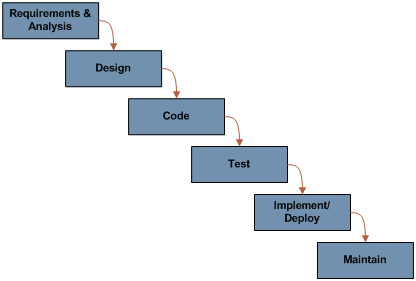
\includegraphics[width=100mm]{images/waterfall.png}
		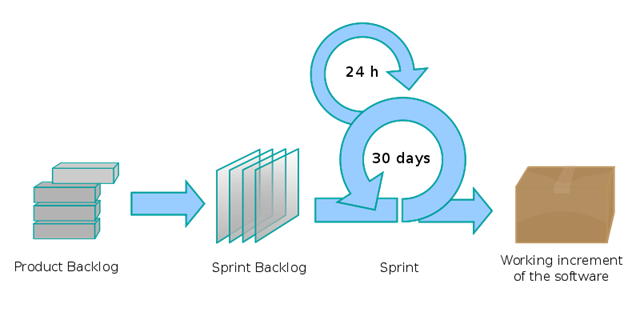
\includegraphics[width=100mm]{images/scrum.png}
		\caption{Software Lifecycles} 
		\label{lifecycles}
	\end{center}
\end{figure}

The project will talk about software lifecycles, and more specifically, how to
implement them in research products. The two major types of software 
developement lifecycles covered in the project are \textbf{Waterfall} (Figure 
\ref{lifecycles} top) and \textbf{Agile Scrum} (Figure \ref{lifecycles} 
bottom). When building HPC / parallel software applications, there are extra
steps that must be done correctly. The project will cover lifecycles in ways
that will maximize usefullness to non - computer scientists.


\subsection{Methodology}

\subsubsection{HPC Cluster}
\label{sec:hpc}

The project will use an HPC cluster as a platform for software. The cluster 
will run Rocks 5.4 for an operating system (OS). Rocks is based off of CentOS 5,
which is a Linux operating system. The cluster will have 1 head node that hosts
a batch server, and the software developed in the project will be submitted as
jobs for the batch server to manage. A scheduler will also be used to help the
batch server schedule jobs. The batch server will be Torque 3.0.0, and the 
scheduler will be Maui 3.3.1 . 

The cluster will then have up to 35 
compute nodes that process this project's software. Each computer node will
have multiple CPU's, and all can potentially be accessed by one compute job.

\begin{figure}[h]
	\begin{center}
	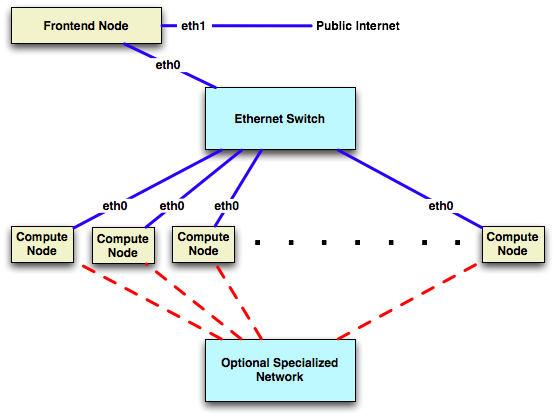
\includegraphics[width=100mm]{images/cluster.png}
	\caption{Rocks Cluster Network Topology \cite{rocks}} 
	\end{center}
\end{figure}

The cluster hardware is a new aquisition in CNR, and is not part of the budget
for this project. Hypothetical cluster run times will be calculated and 
hypothetical budgets will be shown, but no actual budget is needed. 
Although the hardware setup is beyond the scope of the project, the system
description will be necessary to the project software design. Therefore, the 
cluster design will be discussed.

The cluster head node will run a data server either on its head node or as 
another server on the cluster's network. The data server will include a 
Network File System (NFS) server and possibly a MySQL server. The cluster will 
will use environment modules to manage the software needed, so that multiple 
versions of the software can run. 


\pagebreak


\subsubsection{Existing Software}
\label{sec:esoftware}

The project will require the following software:
\begin{itemize}
	\item OpenMPI 1.4.3 (application)
	\item R 2.10.x (language)
	\begin{itemize}
		\item SNOW (library)
		\begin{itemize}
			\item Rmpi (library)
		\end{itemize}
	\end{itemize}
	\item python 2.6
	\begin{itemize}
		\item pyMPI (library)
		\item numpy (library)
		\item scipy (library)
	\end{itemize}
\end{itemize}

\subsubsection{Project Software}

Project software will be software produced by this project. It will either be
parallel improvements of existing software, or it will be new software based
on the project algorithms. The software will be written in R and Python 
languages as listed in Section \ref{sec:esoftware}, and will be 
supplements to the final report. The code content will not be included in the 
report itself.

The project software will be implemented based on Section \ref{sec:hpc}.
The underlying HPC Cluster system affects the methodology of code writing. It 
will be referenced in the project software section as much as needed, so 
non-expert readers can reproduce it on similar systems. 


\pagebreak


\subsection{Annotated Bibliography}
\begin{thebibliography}{99}
\bibitem{gordon_moore} Manek Dubash (2005-04-13). "Moore's Law is dead, says
        Gordon Moore". {\em Techworld}. Retrieved 2006-06-24
	\\
Gordon Moore was an engineer at Intel when CPU's began to become popular. The
processor explosion started, and Moore observed that the amount of transistors
on an IC chip doubled every 2 years. This resulted of a doubling in processing
power that lasted until the late 1990's. Then, engineers simply reached 
physical limitations, in which they had shrunk circuits to the size that they
were counting atoms. Moore's Law, and the end of it, highlights existing 
concerns that processing has been falling behind other technological expanses.

\bibitem{bb} Horne, Garton, et al. "Analyzing Animal Movements using Brownian
        Bridges". { \em Ecology } 88(9) 2007: 2354-2363. Print
	\\
Horne and associates came up with a new approach to creating probability maps
of where animals may be in a habitat, based off of where they had been 
previously. Using Brownian Bridges created a method to do this. Although the 
resulting maps told researches where animals would be, it didn't make any 
direct relations with habitat. The research involves calculations over many locations, which is easily parallelizable.

\bibitem{syn} Horne, Garton, Rachlow. "A synoptic model of animal space use:
        Simultaneous estimation of home range, habitat selection, and
        inter/intra-specific relationships" {\em Ecological Modelling}
        214, 2008: 338-348. Print.
	\\
Horne and associate then moved on to the Synoptic Model for tieing animal 
movement to habitat covariates. From this, any observed animal's behaviors 
could be predicted by its habitat. This lead to current work the author is 
involved with to tie the Brownian Bridge and Synoptic Model together. The
result is a hugely paralellizable application.

\bibitem{james} Foster, James. {\em Visualizing Human Microbiome
	Ecosystems}. University of Idaho: Computer Science Colloquium, 
	December 7th 2010. Seminar.
	\\
James is a strong proponent of interdisciplinary efforts like IBEST, and has
given many talks about the intersect of science and technology. He has degrees
and background in both, and is a great personal source for many scientific
processes and technologies.

\end{thebibliography}


\pagebreak


\section{Workplan}

Parallel Concepts create the basis of understanding the entire project. 
Parallel Concepts will then be applied in simple version of Parallel 
Programming. Once the project has shown concepts implemented in code, the 
research will then focus on taking real world algorithms, and making the same
transfer to parallelism. 

The research will then go on to explain the foundation of parallel programming,
the HPC Cluster. Once completed, the reader will have a solid understanding 
from concepts to implementation, all the way to the HPC Operating System.

Next, the project will talk about how to measure performance of algorithms,
and how to profile software. It will then help readers identify when software
it is appropriate for parallelism.

Finally, the research would summarize everything with explaining Software
Lifecycles. More specifically, how to plan large scale computing projects, 
and how to develop software for HPC / parallel environments. 

\subsection{Schedule}

\begin{tabular}{ l r }
  March 13th - 19th		& Parallel Concepts \\
  March 20th - 26th 		& Parallel Programming \\
  March 27th - April 2nd	& Algorithms \\
  April 3rd - 9th		& HPC Cluster \\
  April 10th - 16th		& Profiling Applications for Parallelism\\
  April 17th - 23rd		& Software Lifecycles \\
  April 24th - 29th		& Proof read, final edits \\
	
\end{tabular}


\section{Statement of Qualifications}
This research project is a collection of tutorials, write up, and general 
thoughts collected in 2+ years working in the University of Idaho IBEST 
Computing Core. It is also information collected and researched in NCMGRP, a
research project lead by Ph. D. student Adam Wells at the University of Idaho 
College of Natural Resources. 

This project content may be included in the final report
in NCMGRP (Northwest Cascades Mountain Goat Research Project), and will 
hopefully be distributed to users of the IBEST Core, as well as to potential 
projects in CNR. The information in the report will be directly cited or 
indirectly sourced from James Foster (IBEST, Co-founder) and Rob Lyon (IBEST,
Lead System Administrator), Adam Wells (UI CNR Ph. D. student), Jon Horne 
(UI CNR), and others within the author's research interests.

This research project is part of the bigger NCMGRP research project. This is
the first funded university research project the author has directly been 
involved with. The research project may have big implication on what research
the author does for graduate studies, if pursued. The author has spent years 
in one realm or another of environment modeling. The computer science 
portion that is the core of this research is the collection of a lot of previos
efforts.

Once this research is completed, research could be continued in the form of 
Artificial Intelligence. Intelligent agents can simulate the behaviors of these
animals in habitat. Modelling habitats, however, takes a lot of computation,
and would be intractable without good practices in HPC and parallel computing.


\section{Conclusion}
The NSF should fund this project, because it is fundemental to establishing 
more successful projects. Many current projects are lacking, because they do
not have the research that would be conducted in this project. This project
will identify and lay the framework for how to process large amounts of 
scientific data. This is a problem that fundamentally affects almost all
current scientific research, but is also one of the least defined areas.
Computer literacy must increase if science will answere the questions of today,
and this project will help achieve that.


%\required{Broader Impacts}
% as in the project summary, broader impacts must be called out separately 
% in the project description.  You may be able to give more specific
% examples, or discuss how you've previously achieved these impacts.
% It should be similar, but not identical, to the Broader Impacts statement
% in the project summary

%\required{Results From Prior NSF Support}
% 5 pages or fewer of the 15 pages for entire description document.
% include results from NSF grants received in the past 5 years.
% if supported by more than one grant, choose the most relevant one
% for each grant, include: NSF award number, amount, dates of
% support, and publications resulting from this research.
% due to space limitations, it is often advisable to use citations rather
% than putting the titles of the publications in the body 
% of this section

% e.g.: "My prior grant, "Uses of Coffee in Mathematical Research" (DMS-0123456, 
% $100,000, 2005-2008), resulted in 3 papers [1],[2],[3], demonstrating..."

% if requesting postdoctoral research salary, a supplemental 1-page document
% called "Postdoc Mentoring Plan" will be required 

